 \documentclass[12pt]{article}

\usepackage{xcolor}
\usepackage{hyperref}
\usepackage{float}
\definecolor{COLOR_MEAN}{HTML}{f0f0f0}
\definecolor{LINK_COLOR}{HTML}{636EFA}
\hypersetup{
	colorlinks=true,
	linkcolor=LINK_COLOR,
	urlcolor=LINK_COLOR,
	citecolor=LINK_COLOR,
}

% if you need to pass options to natbib, use, e.g.:
%     \PassOptionsToPackage{numbers, compress}{natbib}
% before loading neurips_2024


% ready for submission
%\usepackage{neurips_2024}


% to compile a preprint version, e.g., for submission to arXiv, add add the
% [preprint] option:
% \usepackage[preprint]{neurips_2024}


% to compile a camera-ready version, add the [final] option, e.g.:
\usepackage[final]{neurips_2024}


% to avoid loading the natbib package, add option nonatbib:
%    \usepackage[nonatbib]{neurips_2024}


\usepackage[utf8]{inputenc} % allow utf-8 input
\usepackage[T1]{fontenc}    % use 8-bit T1 fonts
\usepackage{hyperref}       % hyperlinks
\usepackage{url}            % simple URL typesetting
\usepackage{booktabs}       % professional-quality tables
\usepackage{amsfonts}       % blackboard math symbols
\usepackage{nicefrac}       % compact symbols for 1/2, etc.
\usepackage{microtype}      % microtypography
\usepackage[dvipsnames]{xcolor}
\usepackage{tabularx}
\usepackage{booktabs}
\usepackage{amsmath}
\usepackage{listings}
\usepackage{subcaption}
\usepackage[ruled,vlined,linesnumbered,noresetcount]{algorithm2e}
\usepackage{dsfont}
\usepackage{booktabs}
\usepackage{tablefootnote}




\title{Cassava Leaf Disease Classification}


% The \author macro works with any number of authors. There are two commands
% used to separate the names and addresses of multiple authors: \And and \AND.
%
% Using \And between authors leaves it to LaTeX to determine where to break the
% lines. Using \AND forces a line break at that point. So, if LaTeX puts 3 of 4
% authors names on the first line, and the last on the second line, try using
% \AND instead of \And before the third author name.


\author{%
	Anusha Agarwal\thanks{Equal contribution. Listing order is alphabetical.} \hspace{1em} Fanyi Pu\footnotemark[1] \hspace{1em} Gordon Tian Xiao Chen\footnotemark[1] \hspace{1em} Siyang Shao\footnotemark[1] \hspace{1em} Yi Shan\footnotemark[1] \\
	College of Computing and Data Science\\
	Nanyang Technological University\\
	Singapore 639798 \\
	\texttt{\{ANUSHA009, FPU001, GCHEN019, SHAO0054, SH0005YI\}@e.ntu.edu.sg} \\
}

\usepackage{graphicx}

\newcommand{\VIT}{\textsc{ViT}\xspace}
\newcommand{\VITFULL}{\textsc{Vision Transformer}\xspace}
\newcommand{\CROP}{\textsc{Cropnet}\xspace}
\newcommand{\CONV}{\textsc{ConvNeXtV2}\xspace}


\lstset{ 
  language=python,                     % the language of the code
  basicstyle=\ttfamily, % the size of the fonts that are used for the code
  numbers=left,                   % where to put the line-numbers
  numberstyle=\color{Blue},  % the style that is used for the line-numbers
  stepnumber=1,                   % the step between two line-numbers. If it is 1, each line
                                  % will be numbered
  numbersep=5pt,                  % how far the line-numbers are from the code
  backgroundcolor=\color{white},  % choose the background color. You must add \usepackage{color}
  showspaces=false,               % show spaces adding particular underscores
  showstringspaces=false,         % underline spaces within strings
  showtabs=false,                 % show tabs within strings adding particular underscores
  frame=single,                   % adds a frame around the code
  rulecolor=\color{black},        % if not set, the frame-color may be changed on line-breaks within not-black text (e.g. commens (green here))
  tabsize=2,                      % sets default tabsize to 2 spaces
  captionpos=b,                   % sets the caption-position to bottom
  breaklines=true,                % sets automatic line breaking
  breakatwhitespace=false,        % sets if automatic breaks should only happen at whitespace
  keywordstyle=\color{RoyalBlue},      % keyword style
  commentstyle=\color{YellowGreen},   % comment style
  stringstyle=\color{ForestGreen}      % string literal style
} 

\begin{document}
	
	\begin{titlepage}
	\begin{figure}[!t]
		\centering
		
\includegraphics[width = 4.3in]{title/logo.pdf}
	\end{figure}

	\centering
	\huge{\textbf{SC4000: Machine Learning}}\\[0.2in]
	\huge{\textbf{Project Report}}\\[2in]

	%	\LARGE{\textbf{YOUR NAME}}\\
	%	\normalsize{Matriculation number}\\[0.2in]

	\begin{table}[h]
		\centering
		\resizebox{\textwidth}{!}{%
			\begin{tabular}{lll}
				\toprule
				\textbf{Name} & \textbf{Email} & \textbf{Matric Number} \\
				\midrule
				Pu Fanyi & \texttt{FPU001@e.ntu.edu.sg} & \texttt{U2220175K} \\
                Agarwal Anusha & \texttt{ANUSHA009@e.ntu.edu.sg} & \texttt{U2023105H} \\
				Chen Gordon Tian Xiao & \texttt{GCHEN019@e.ntu.edu.sg} & \texttt{U2140820A} \\
				Shan Yi & \texttt{SH0005YI@e.ntu.edu.sg} & \texttt{U2222846C}\\
                Shao Siyang &\texttt{SHAO0054@e.ntu.edu.sg}&\texttt{U2120544F}\\
				\bottomrule
			\end{tabular}%
		}
	\end{table}

	\Large{Course Coordinator: Asst Prof Ke Yiping, Kelly}\\[0.5in]

	%	\large{A Final Year Report submitted to Asian School of the Environment, Nanyang Technological University in partial fulfilment of the requirements for the Degree of }\\[0.1in]

	\LARGE{College of Computing and Data Science}\\
	\LARGE{Nanyang Technological University, Singapore}\\[0.3in]


	\LARGE{2024/2025 Semester 1}
	\newpage
\end{titlepage}

	\newpage
	
	
	\maketitle
	
	
    \begin{abstract}
With the advent of the 2020s AI era, it seems that all efforts have been focused on Transformers. However, we believe ResNet still holds its place. By leveraging a voting mechanism between ResNet and Transformer architectures, we may achieve different results. We propose a new model voting method to add a dimension for voting. In the Kaggle Cassava Leaf Disease Classification competition, our model achieved rank $4 / 3901$ on the Public Benchmark and rank $2 / 3901$ on the Private Benchmark. Our training code can be found in \href{https://github.com/pufanyi/SC4000}{GitHub} and all our models can be found in \href{https://huggingface.co/collections/pufanyi/sc4000-6717aaebf10b0e67e9a34a0d}{Hugging Face}.
\end{abstract}


    \section{Introduction}

As outlined in the competition overview \cite{cassava-leaf-disease-classification}, cassava is an important crop in Africa, but its yields are significantly affected by diseases. The current disease monitoring primarily relies on visual inspection by agricultural experts, which is labor-intensive and costly. Thus, it is essential to identify common cassava diseases to address this issue. As illustrated in Fig.~\ref{CassavaDisease}, there are four main types of cassava diseases: Bacterial Blight, Brown Streak Disease, Green Mottle, and Mosaic Disease. Each disease displays distinct characteristics on the leaves, allowing for differentiation from healthy cassava leaves through image classifiers.

Bacterial Blight (Fig.~\ref{CassavaFigBac}) is characterized by dead leaf spots surrounded by yellow halos \cite{uwm2024BacterialBlight}. Brown Streak Disease (Fig.~\ref{CassavaFigBro}) presents as patches of yellow intermingled with the standard green color of the leaves \cite{patil2015cassava}. Green Mottle Disease (Fig.~\ref{CassavaFigGreen}) is identifiable by green spots on the leaves that appear as if they were painted on \cite{robson2024cassava}. Lastly, Mosaic Disease (Fig.~\ref{CassavaFigMos}) results in symptoms such as discoloration, with leaves showcasing variations of yellow, white, light, and dark shades \cite{chikoti2019cassava}.

\begin{figure}[htbp]
    \centering
    \begin{subfigure}{0.24\textwidth}
        \centering
        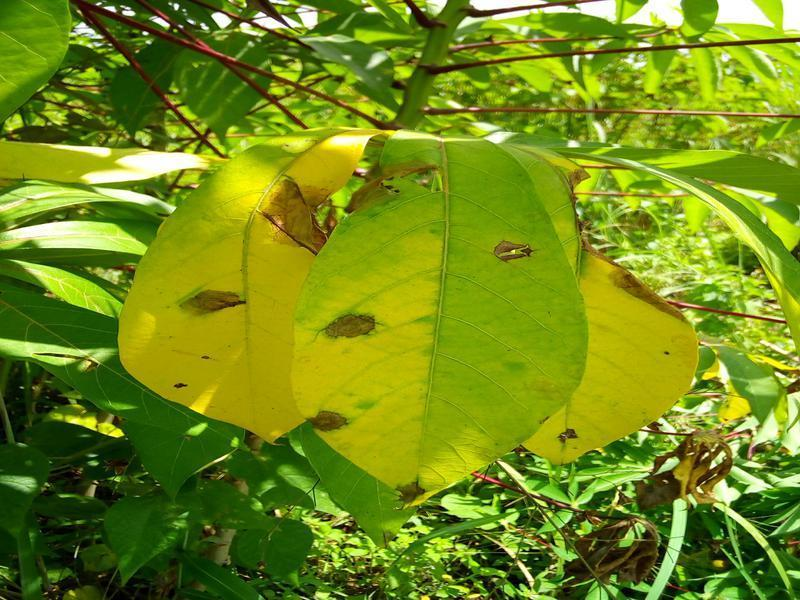
\includegraphics[width=\linewidth]{graphs/DiseaseImage/BacterialBlight.jpg}
        \caption{Bacterial Blight}
        \label{CassavaFigBac}
    \end{subfigure}
    \begin{subfigure}{0.24\textwidth}
        \centering
        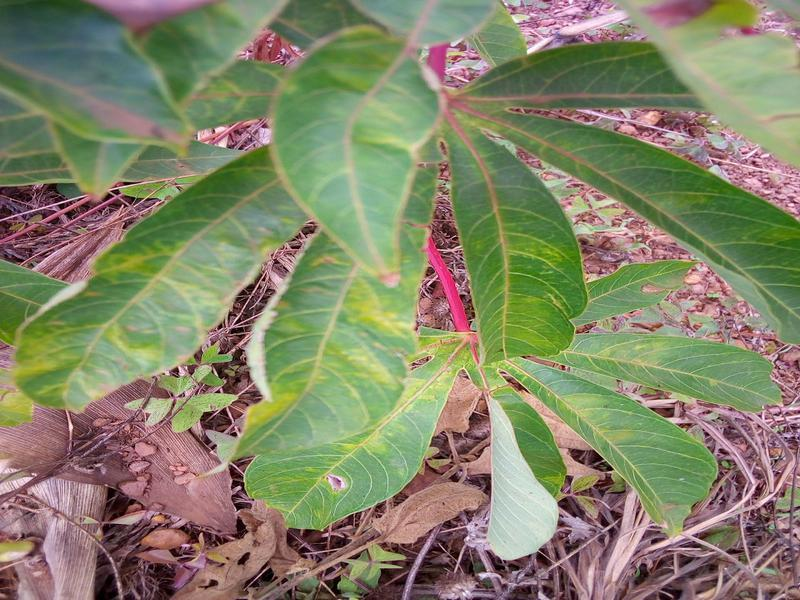
\includegraphics[width=\linewidth]{graphs/DiseaseImage/BrownStreak.jpg}
        \caption{Brown Streak}
        \label{CassavaFigBro}
    \end{subfigure}
    \begin{subfigure}{0.24\textwidth}
        \centering
        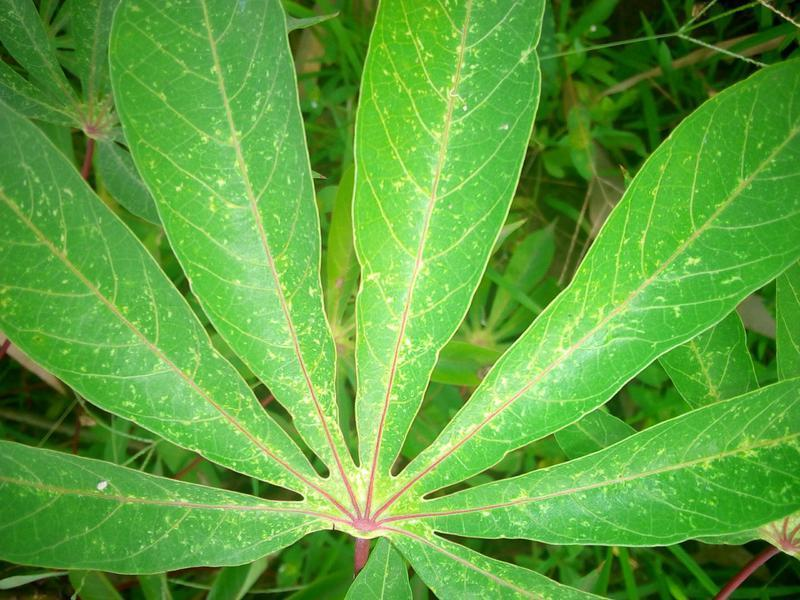
\includegraphics[width=\linewidth]{graphs/DiseaseImage/GreenMottle.jpg}
        \caption{Green Mottle}
        \label{CassavaFigGreen}
    \end{subfigure}
        \begin{subfigure}{0.24\textwidth}
        \centering
        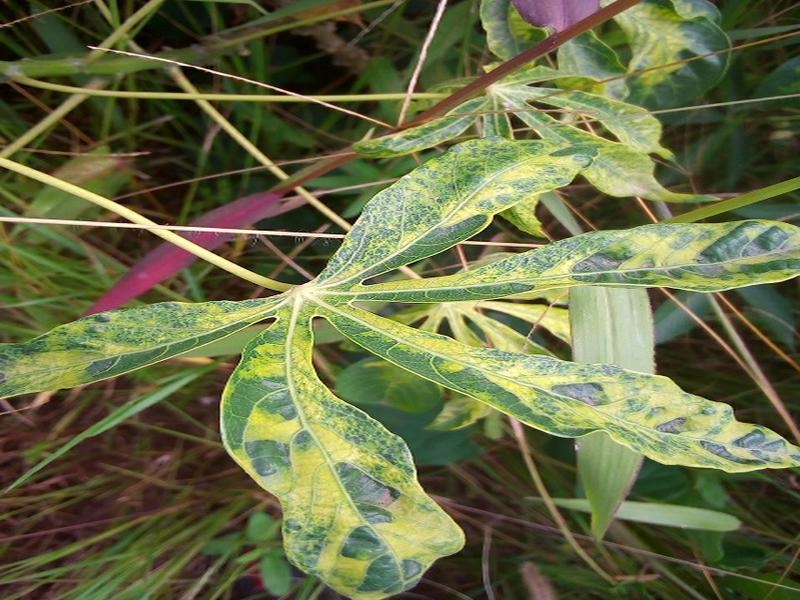
\includegraphics[width=\linewidth]{graphs/DiseaseImage/Mosaic.jpg}
        \caption{Mosaic}
        \label{CassavaFigMos}
    \end{subfigure}
    \caption{Cassava Disease Type}
    \label{CassavaDisease}
\end{figure}

The task aims to classify cassava leaf images based on the input data, to determine whether the leaf is healthy or infected by a specific type of virus illustrated before. Specifically, the input consists of image data with a resolution of $800 \times 600$ pixels, and the output is a category label indicating the leaf's condition. We categorize diseases from types $0$ to $3$ as Bacterial Blight through Mosaic and use category $4$ to label healthy cassava leaf images.

There are several challenges in the task. First, the original dataset has a significant class imbalance, with many more samples available for the Mosaic disease type than for the others. This imbalance can lead to biased model predictions, where the classifier favors the majority classes and underperforms the minority classes. Second, our analysis shows that a single model struggles to accurately capture and differentiate the characteristics of all virus types due to subtle visual differences among some categories. To address these challenges and improve overall classification performance, it is necessary to use strategies such as data augmentation, re-sampling techniques, and model fusion. 

Our dataset comes from the public dataset on Kaggles~\cite{cassava-leaf-disease-classification}, which includes $21367$ labeled images during routine surveys conducted in Uganda. These images were captured by the farmers in their cassava gardens, which show real-world scenarios to distinguish different kinds of diseases.

    \section{Data Cleaning and Processing}
This section details the steps undertaken to prepare the dataset for training and testing the Cassava Leaf Disease Classification model. The dataset was analyzed, cleaned, and processed to ensure proper training and evaluation. 

\subsection{\textbf{Exploratory Data Analysis (EDA)}}
The dataset initially contained 21,397 images categorized into five classes. Analysis of the training dataset revealed the following class distribution shown in Figure~\ref{fig:ImbalancedData}.

\begin{figure}[t]
    \centering
    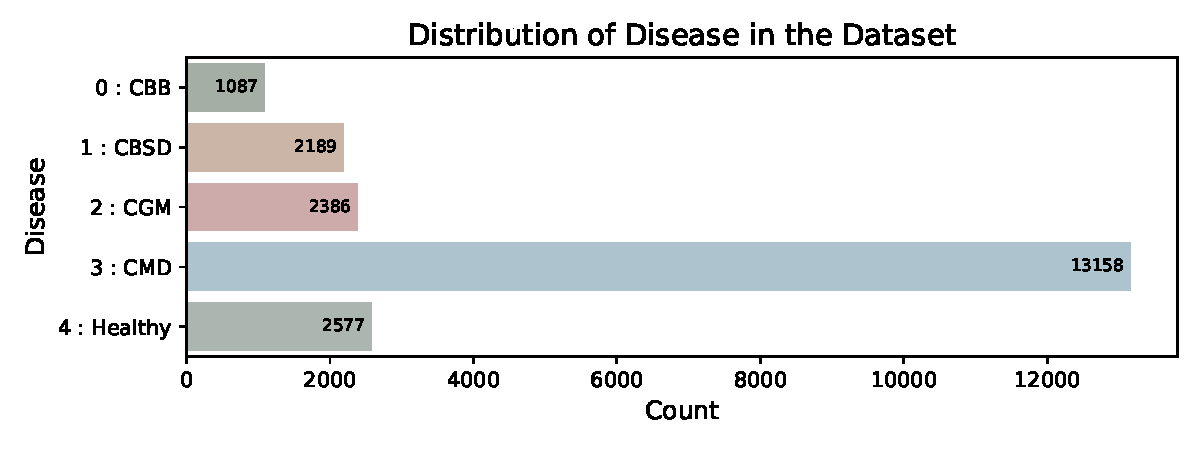
\includegraphics[width=1\linewidth]{graphs/overview/Distribution of Disease in the Dataset.pdf}
    \caption{Imbalanced Cassava Disease Label Distribution}
    \label{fig:ImbalancedData}
\end{figure}

Figure~\ref{fig:ImbalancedData} highlighted a significant class imbalance, with Label 3 accounting for over 60\% of the dataset, while Label 0 represented only 5\%. To address this imbalance and explore its impact on the model’s performance, two dataset preparation strategies were employed: Balanced Data and Imbalanced Data with Train-Validation Split.

\subsection{\textbf{Dataset Preparation }}
\subsubsection{Balancing the Data}

To address the class imbalance in the training dataset, a validation set of 500 samples was created by randomly sampling 100 images from each class.
The remaining samples were allocated to the training set, resulting in the new distribution shown in Figure~\ref{fig:BalancedDataset}.

\begin{itemize}
    \item \textbf{Train Set:} 20,897 samples.
    \item \textbf{Validation Set:} 500 samples.
    \item \textbf{Test Set:} 1 sample (reserved for evaluation consistency).
\end{itemize}

\begin{figure}[t]
    \centering
    \begin{subfigure}{0.4\textwidth}
        \centering
        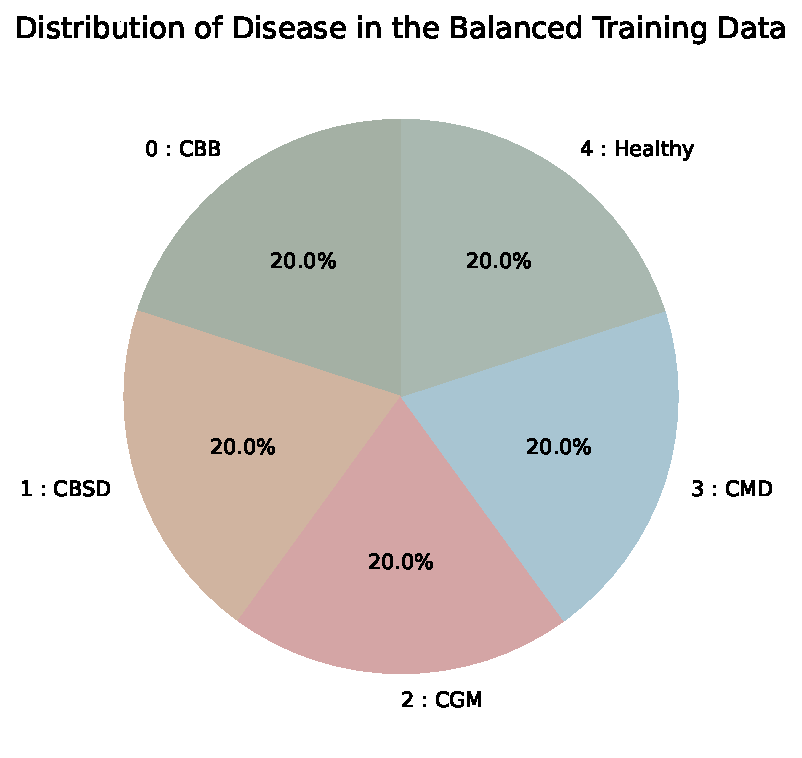
\includegraphics[width=\linewidth]{graphs/overview/Distribution of Disease in the Balanced Training Data.pdf}
        \caption{Balanced Train Dataset}
        \label{fig:BalancedTrain}
    \end{subfigure}
    \begin{subfigure}{0.4\textwidth}
        \centering
        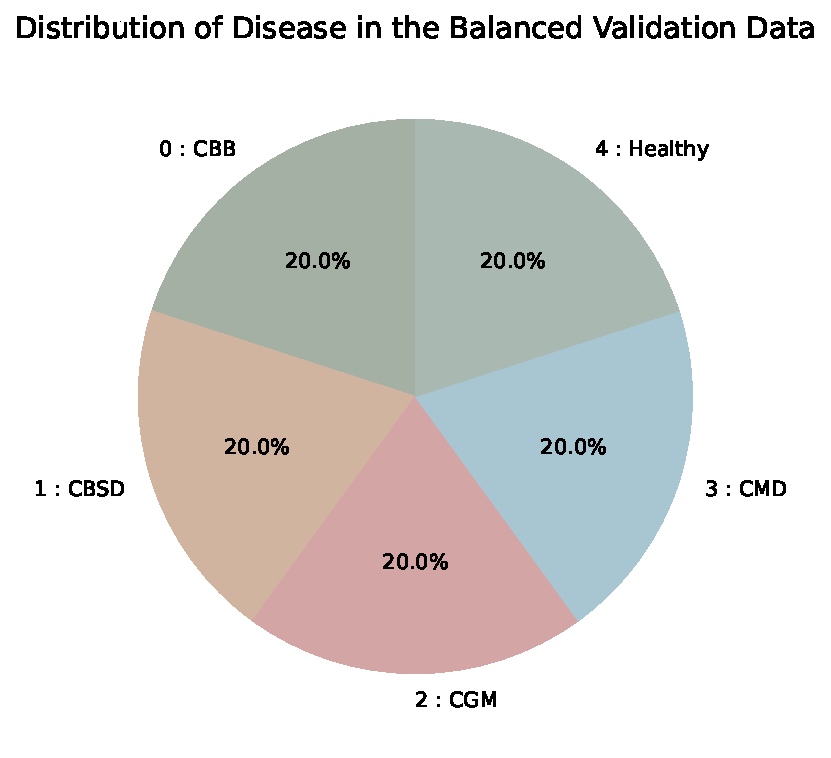
\includegraphics[width=\linewidth]{graphs/overview/Distribution of Disease in the Balanced Validation Data.pdf}
        \caption{Balanced Val Dataset}
        \label{fig:BalancedVal}
    \end{subfigure}
    \caption{Balanced Cassava Disease Label Distribution}
    \label{fig:BalancedDataset}
\end{figure} 

The training data was further balanced by down-sampling all classes to the size of the smallest class (\textbf{987 samples}). This ensured an equal representation of all classes as seen in Figure[\ref{fig:BalancedDataset}]

By addressing the imbalance, this approach aims to ensure that the model receives equal exposure to all classes during training. This is particularly beneficial for smaller classes that might otherwise be under-represented.

\subsubsection{Train-Validation Split with Imbalanced Data}
To maintain the original class distribution, a separate train-validation split was performed without balancing the dataset:

\begin{itemize}
    \item \textbf{Train Set:} 95\% of the dataset (\textbf{20,327 samples}).
    \item \textbf{Validation Set:} 5\% of the dataset (\textbf{1,070 samples}).
    \item \textbf{Test Set:} 1 sample.
\end{itemize}

The distribution is described in Figure~\ref{fig:TrainValSplit}. This split allows the model to learn from the imbalanced distribution, simulating a real-world scenario where imbalances exist. Maintaining the imbalance is essential to evaluate how the model performs without any balancing techniques applied.


\begin{figure}[t]
    \centering
    \begin{subfigure}{0.4\textwidth}
        \centering
        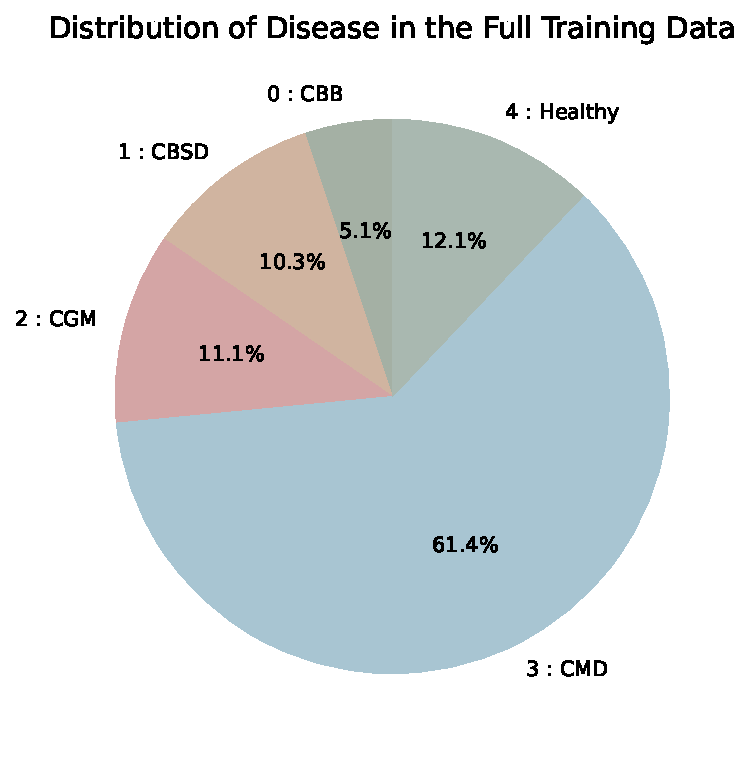
\includegraphics[width=\linewidth]{graphs/overview/Distribution of Disease in the Full Training Data.pdf}
        \caption{Train Dataset 95\%}
        \label{fig:ImbalancedTrain}
    \end{subfigure}
    \begin{subfigure}{0.4\textwidth}
        \centering
        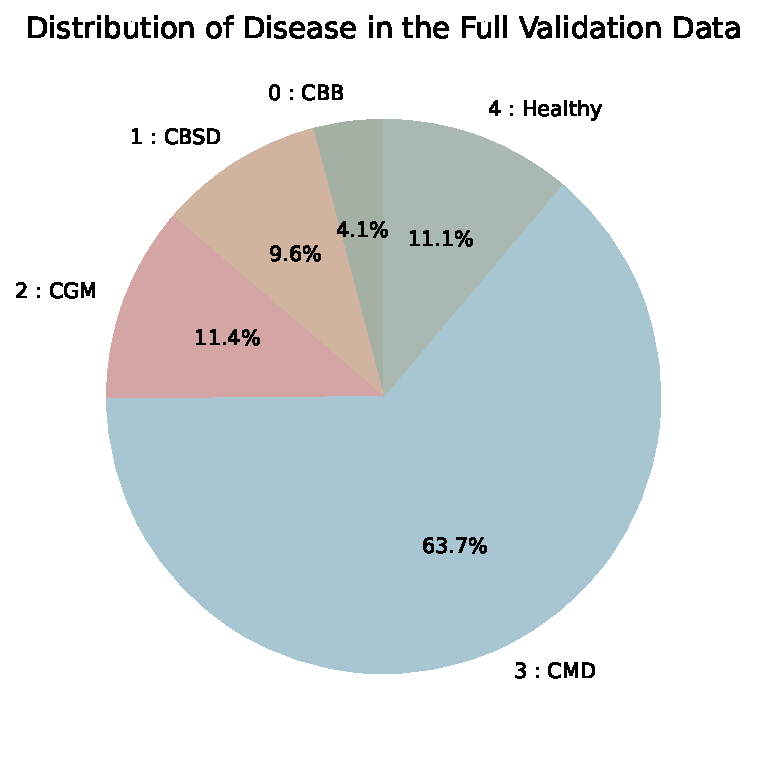
\includegraphics[width=\linewidth]{graphs/overview/Distribution of Disease in the Full Validation Data.pdf}
        \caption{Val Dataset 5\%}
        \label{fig:ImbalancedVal}
    \end{subfigure}
    \caption{Train-Val Split Cassava Disease Label Distribution for the Full Dataset}
    \label{fig:TrainValSplit}
\end{figure} 



\subsection{Data Augmentation}

Data augmentation is a crucial technique in computer vision that is used to enhance the diversity of the training dataset without the need to collect additional data. It helps improve the model's generalization ability by simulating real-world variations, such as changes in orientation, scale, lighting, and color. For this analysis, data augmentation was applied to the training dataset to make the model robust to noise and variations in cassava leaf images.

\subsubsection{Preprocessing Steps for Training}\label{sec:pre_image}
Focused on increasing dataset variability through augmentation (e.g., random rotations, flips, and color jitter) to improve the model's generalization ability and robustness. The detailed reason we do this is described in Section~\ref{sec:overfit}.

The following augmentation techniques were applied during the training phase:

\begin{itemize}
    \item \textbf{Random Rotation:} The images were randomly rotated by up to 45 degrees to account for variations in orientation.
    \item \textbf{Random Resized Crop:} Images were randomly cropped and resized to ensure consistent input size while preserving variability in the content.
    \item \textbf{Random Horizontal Flip:} Horizontal flipping of images was performed to simulate variations in leaf direction.
    \item \textbf{Random Vertical Flip:} Vertical flipping was applied to enhance the diversity of leaf orientations in the training data.
    \item \textbf{Color Jitter:} Random adjustments were made to the brightness, contrast, saturation, and hue of images to account for variations in lighting and color conditions.
    \item \textbf{ToTensor:} The ToTensor transformation was applied to convert the augmented images into PyTorch tensors, ensuring compatibility with deep learning models.
    \item \textbf{Normalization:} Finally, the images were normalized using the mean and standard deviation values obtained from the pretrained image processor. This scales pixel values to a standard range, aiding in faster convergence during training.
\end{itemize}

These transformations were applied during the training phase using the following pipeline:



\begin{lstlisting}
self.train_transforms = Compose(
  [
    RandomRotation(degrees=45),
    RandomResizedCrop(size),
    RandomHorizontalFlip(),
    RandomVerticalFlip(),
    ColorJitter(brightness=0.1, contrast=0.1, saturation=0.1, hue=0.1),
    ToTensor(),
    normalize,
  ]
)
\end{lstlisting}

\begin{figure}[t]
    \centering
    % 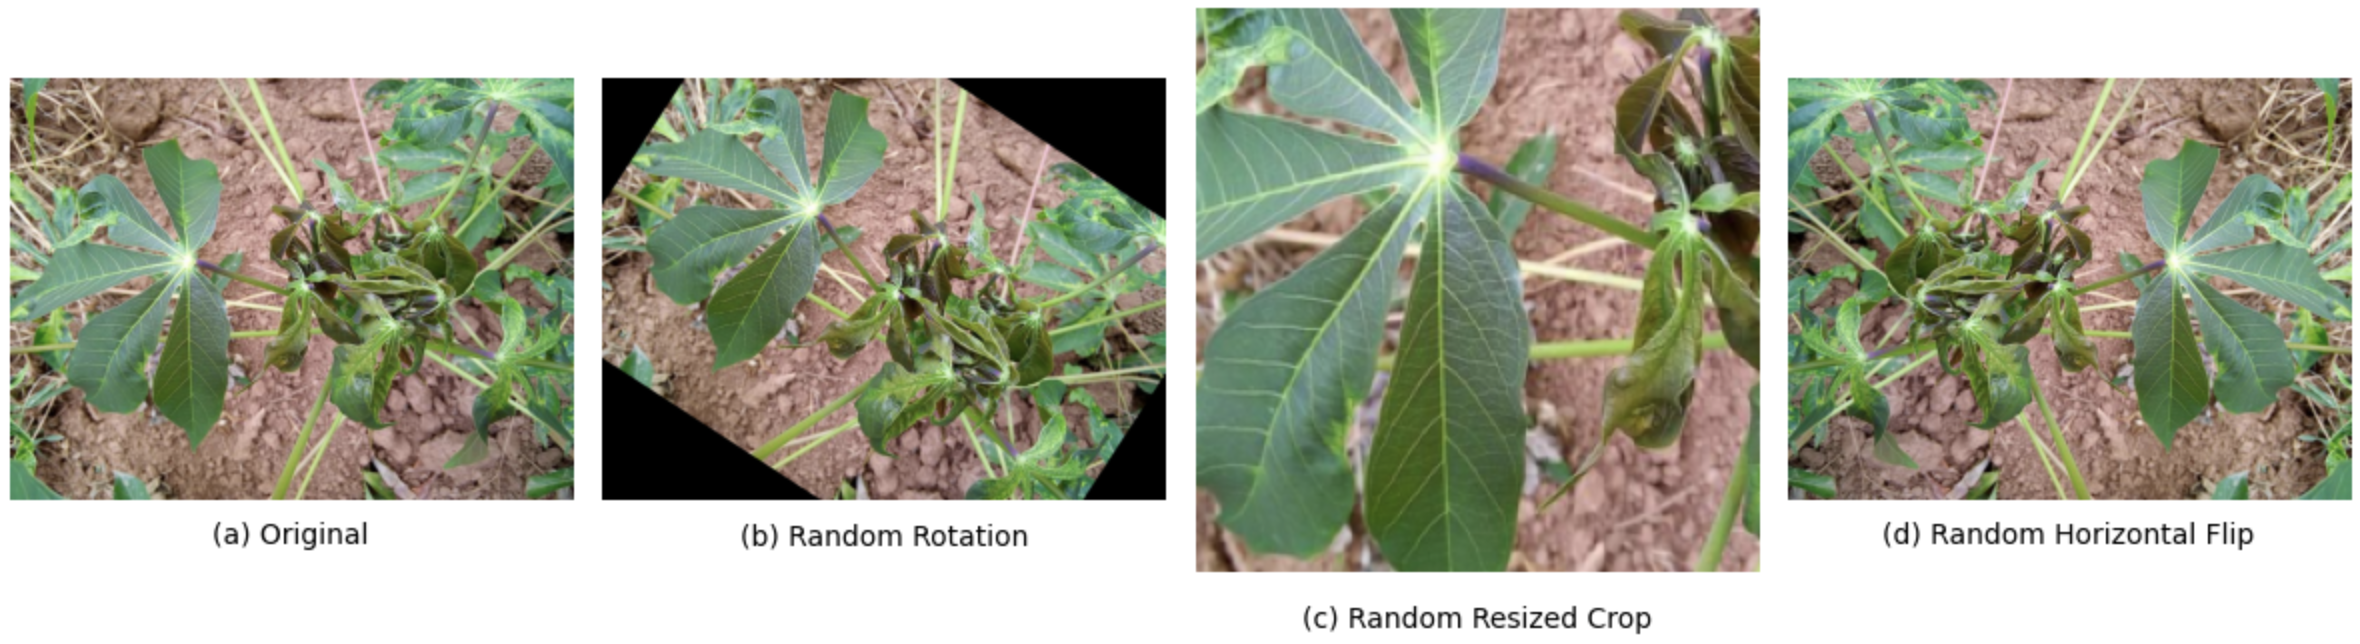
\includegraphics[width=1.0\linewidth]{graphs/TrainDataAug1.png}
    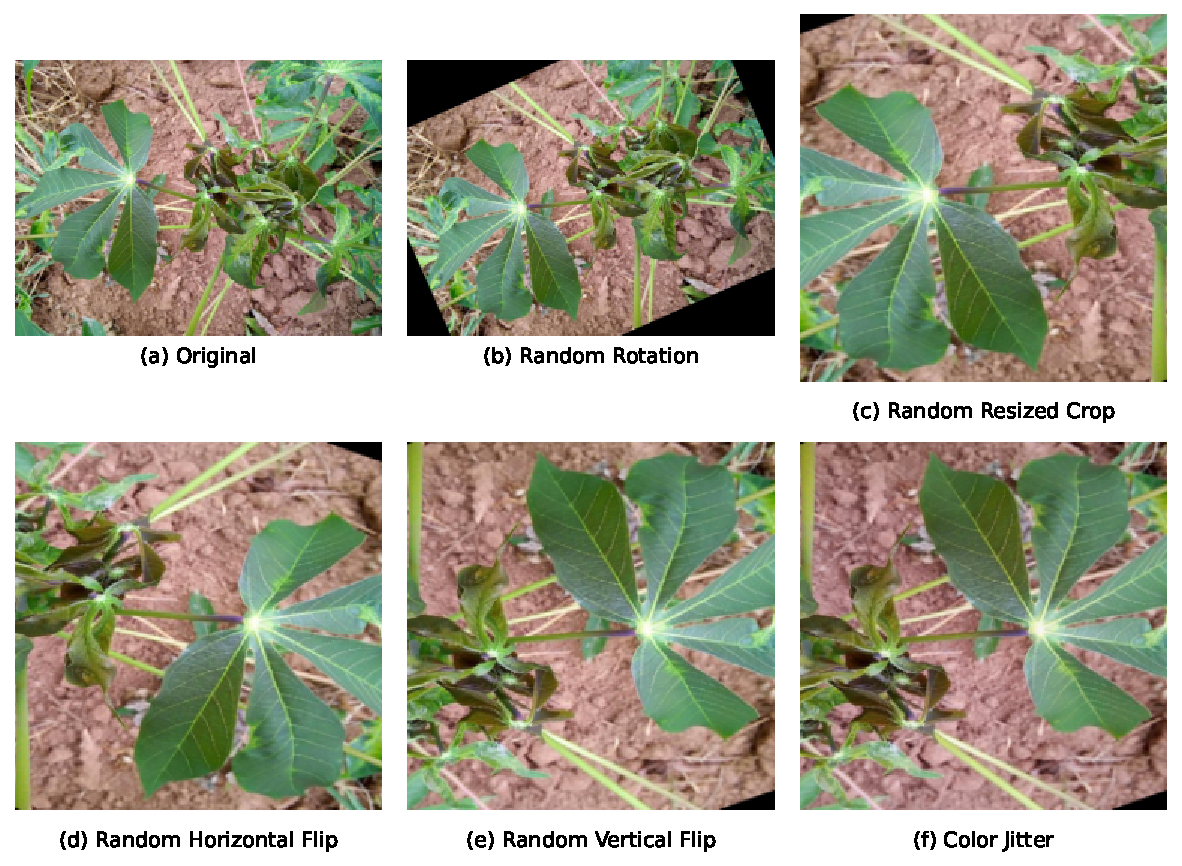
\includegraphics[width=1.0\linewidth]{graphs/overview/TrainTransform.pdf}
    % \centering
    % 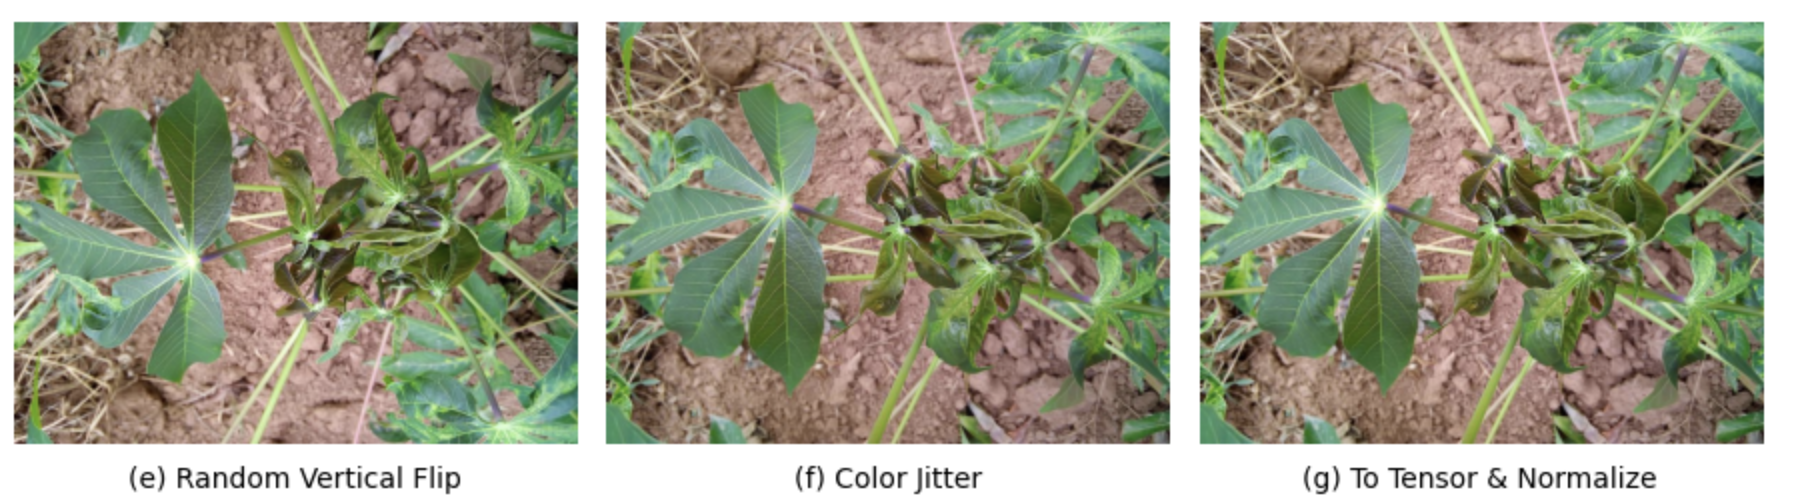
\includegraphics[width=0.8\linewidth]{graphs/TrainDataAug2.png}
    \caption{Data Augmentation on Train Sample}
    \label{fig:TrainAug2}
\end{figure}

To better understand the impact of data augmentation, visualization was performed on the transformations applied to a sample image from the training dataset. Each transformation demonstrates how the training data is modified to improve the model's robustness and generalization as seen in Figure~\ref{fig:TrainAug2}.

\subsubsection{Preprocessing Steps for Validation}

In contrast to the training dataset, the validation dataset underwent simpler preprocessing steps designed to preprocess the images uniformly without augmentation. Although each model has its own image processor, we decided to redefine image processing to ensure the correct order of transformations. This ensures that the evaluation reflects how the model performs on real-world, unaltered images:
\begin{itemize}
    \item \textbf{Resize:} Images were resized to match the input size expected by the model.
    \item \textbf{Center Crop:} A center crop ensured that the main content of the image remained intact while maintaining uniform input dimensions.
    \item \textbf{ToTensor:} Like the training dataset, the validation images were converted into PyTorch tensors to facilitate model compatibility.
    \item \textbf{Normalization:} The same normalization parameters (mean and standard deviation) as used in the training dataset were applied to maintain consistency.
\end{itemize}

For validation, a simpler transformation pipeline was used to standardize the input images:

\begin{lstlisting}
self.val_transforms = Compose(
  [
    Resize(size),
    CenterCrop(size),
    ToTensor(),
    normalize,
  ]
)
\end{lstlisting}

\begin{figure}[t]
    \centering
    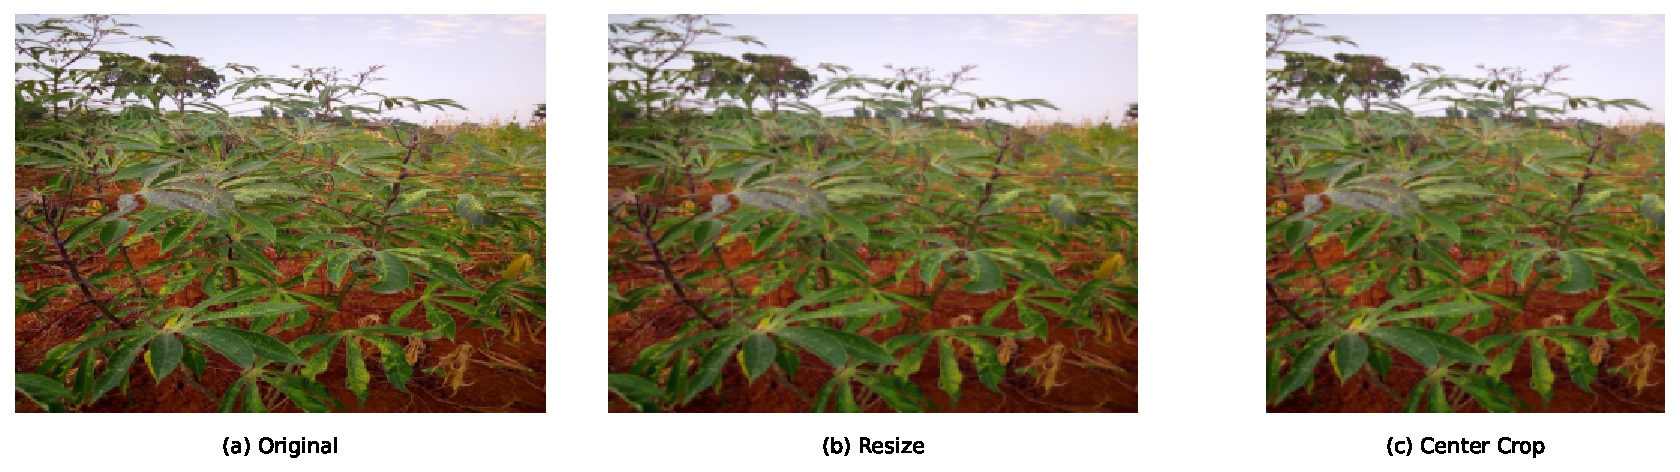
\includegraphics[width=\linewidth]{graphs/overview/ValidationTransform.pdf}
    \caption{Data Augmentation on Val Sample}
    \label{fig:ValDataAug}
\end{figure}

A similar visualization is seen for each step performed in the transformation standardization pipeline for validation data in Figure~\ref{fig:ValDataAug}.

Data augmentation during training enhances the model's ability to generalize, while simpler validation preprocessing ensures consistent and unbiased evaluation of the model's performance. This dual approach strikes a balance between robustness and reliability.

\subsubsection{Further Improvement: Reducing noise with Segment Anything Model}

Most images contain irrelevant background details, such as dirt or leaves from other species, which can introduce localized noise. To address this during preprocessing, we utilize the Segment Anything Model (SAM), an efficient tool for predicting object masks from images and input prompts.

\begin{figure}[H]
    \centering
    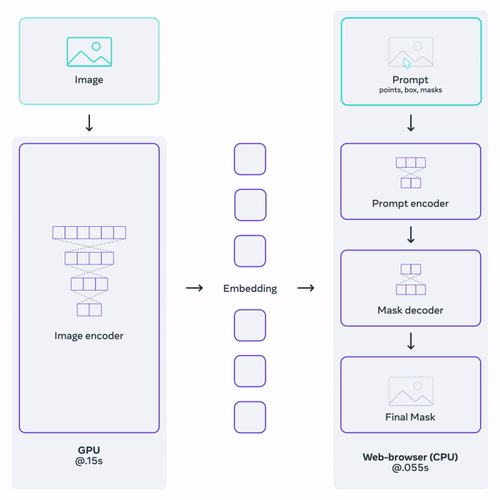
\includegraphics[scale=0.5]{graphs/SAM.jpg}
    \caption{Segment Anything Model Pipeline (Source: Section 3.1c https://segment-anything.com/)}
    \label{fig:SAM}
\end{figure}

Figure \ref{fig:SAM} illustrates how the Segment Anything Model (SAM) operates. SAM uses an image encoder to extract image embeddings and a prompt encoder to process various input prompts, including point coordinates, bounding boxes, and low-resolution masks. The encoded prompts are combined with image embeddings and passed to a mask decoder, which produces the final object masks.

To enable segmentation guided by natural language prompts, we use GroundingDino in conjunction with SAM. GroundingDino is a text-to-bounding-box model that allows users to input an image and a text prompt. It performs zero-shot text-to-bounding-box object detection, effectively identifying objects of interest in an image based on natural language descriptions. The resulting bounding boxes serve as input prompts for SAM, which refines them into accurate segmentation masks.


\begin{figure}[t]
    \centering
    \begin{subfigure}[b]{0.22\linewidth}
        \centering
        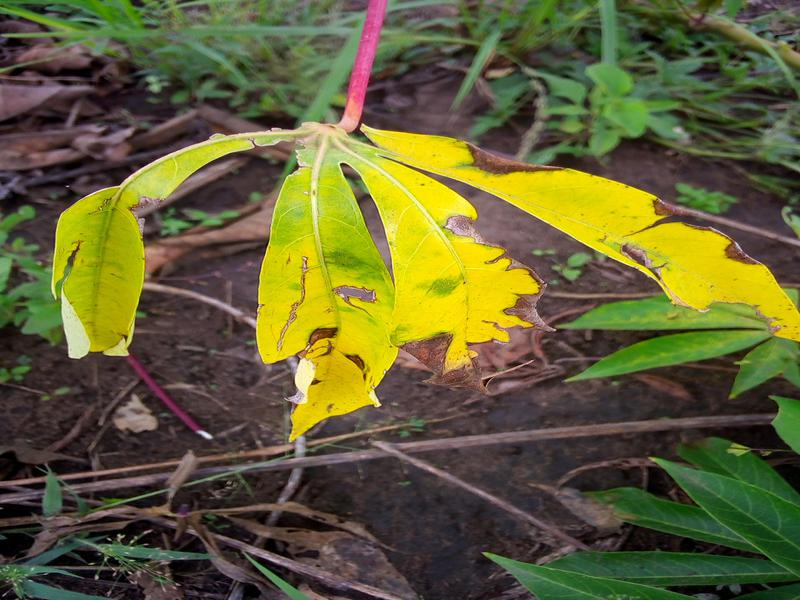
\includegraphics[width=\linewidth]{graphs/samraw1.png}
        \caption{Original Image I}
        \label{fig:Original Image (1)}
    \end{subfigure}
    \hfill
    \begin{subfigure}[b]{0.22\linewidth}
        \centering
        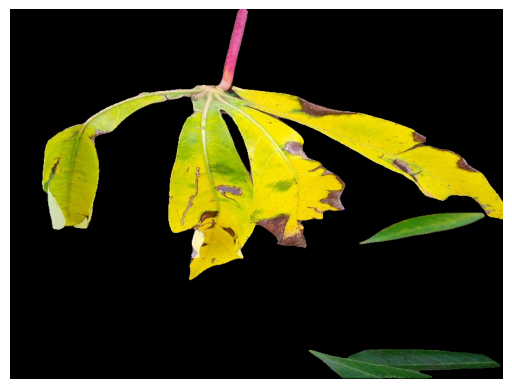
\includegraphics[width=\linewidth]{graphs/sam1.png}
        \caption{Image Mask I}
        \label{fig:Segmentation mask (1)}
    \end{subfigure}
    \hfill
    \begin{subfigure}[b]{0.22\linewidth}
        \centering
        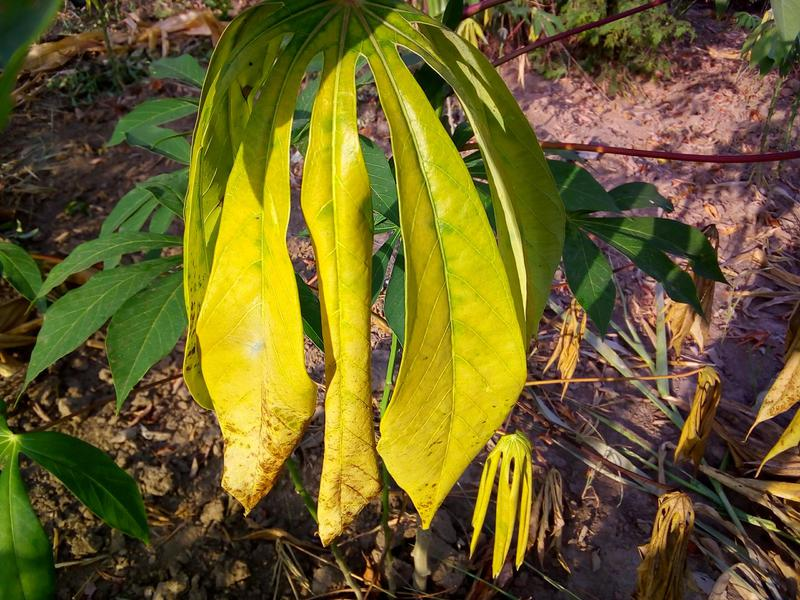
\includegraphics[width=\linewidth]{graphs/samraw2.jpg}
        \caption{Original Image II}
        \label{fig:Original Image (2)}
    \end{subfigure}
     \hfill
     \begin{subfigure}[b]{0.22\linewidth}
        \centering
        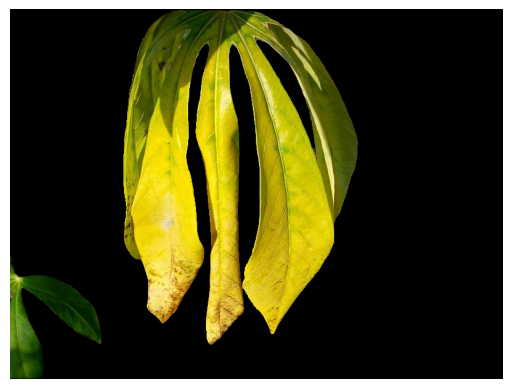
\includegraphics[width=\linewidth]{graphs/sam2.png}
        \caption{Image Mask II}
        \label{fig:Segmentation mask (2)}
    \end{subfigure}
    \caption{Segmentation Masks obtained using Segment Anything Model (SAM)}
    \label{fig:four_images}
\end{figure}

Figure \ref{fig:four_images} illustrates the image before and after processing with SAM. The inverse mask is blacked out to eliminate irrelevant features that contribute to noise. In rare instances where no mask is generated, the entire image is preserved without modifications instead of applying blacking out.

       \section{Model Construction}

\subsection{Model Selection}

Given the high complexity of this classification problem, we aim to conserve computational resources by avoiding retraining the model from scratch. Instead, we perform fine-tuning on multiple models separately and integrate their results to complete the experiments.

\paragraph{\VITFULL} In recent years, the Transformers \cite{vaswani2017attention} architecture has demonstrated remarkable superiority in various vision tasks. Therefore, we plan to use \VITFULL (\VIT) \cite{dosovitskiy2020vit} as one of our training models. We conducted small-scale fine-tuning experiments on models with varying sizes and resolutions using limited data.

Our findings show that, for \VIT, increasing model size and resolution makes the model have a better performance. As a result, we choose \VIT Large model with resolution $384\times 384$\footnote{Obtained from \url{https://huggingface.co/google/vit-large-patch16-384}.} as our pretraining model.

\paragraph{\CONV} According to \cite{liu2022convnet}, although \textsc{Transformers} perform exceptionally well on a wide range of tasks, ResNet \cite{he2016deep} can be ``modernized'' to compete with Transformers in vision tasks. To increase model diversity, we chose \CONV \cite{woo2023convnext}, a purely convolution-based model, as the second pretraining model.

After some small-scale experiments, we found that model size seems to have minimal impact on performance. However, higher resolution significantly improved the model's effectiveness. Based on this, we decided to select the \CONV Base model with resolution $384\times 384$\footnote{Obtained from \url{https://huggingface.co/facebook/convnextv2-base-22k-384}.} as the final pretraining model, as it offers a smaller model size with a higher resolution. This choice maximizes computational efficiency without compromising model performance.

\paragraph{\CROP} We selected \CROP, using \textsc{MobileNetV3} \cite{howard2019searching} as the base architecture and has been trained on the \textit{iNaturalist and plants} subset of ImageNet-21K \cite{deng2009imagenet}. This provides the model with a wealth of knowledge about plant diseases. We further fine-tuned it to achieve better performance. Additionally, the relatively simple architecture of \textsc{MobileNetV3} allowed us to improve training efficiency.

\subsection{Loss Function}

Cross Entropy loss has been proven to be an excellent loss function for classification tasks. We use cross entropy as the initial loss function with minor modifications.

\paragraph{Label Smoothing} Considering that this task involves extensive knowledge in botany and medicine, with high similarity between images of different categories, which often require experts for accurate identification, we propose using label smoothing \cite{Szegedy_2016_CVPR} to reduce the model's over-confidence and improve its calibration \cite{muller2019does}. With label smoothing coefficient $\alpha$, we define the new loss function

\begin{equation}\label{eq:full_loss}
\mathcal{L}(\hat{p}, y)=-\left[(1-\alpha)\log p_y + \alpha\cdot\frac{1}{C}\sum_{c=1}^C\log p_c\right]
\end{equation}

where $\hat{p}$ is the predicted probabilities for each class, $y$ is the answer, $C$ is the number of classes.

In our actual training process, we have $\alpha=0.06$.

\paragraph{Balanced Cross Entropy}

As mentioned in Figure~\ref{fig:ImbalancedData}, our training data is imbalanced. Although downsampling is a reasonable approach to balancing the dataset, this method leads to the loss of a significant amount of valuable training data. Inspired by \cite{aurelio2019learning}, we decided to try changing the loss to

\begin{equation}\label{eq:balanced_loss}
\mathcal{L}(\hat{p}, y)=-w_y\cdot\left[(1-\alpha)\log p_y + \alpha\cdot\frac{1}{C}\sum_{i=c}^C\log p_c\right]
\end{equation}

And the weight vector $w$ is defined as

\begin{equation}
w_c = \frac{n}{C \cdot \sum_{i=1}^n\mathds{1}_{y_i=c}}
\end{equation}

where $n$ is the number of training data.

In Equation \ref{eq:balanced_loss}, data with smaller quantities holds a higher weight in the loss calculation, causing the model to pay more attention to this subset during training. However, the drawback of this approach is that it no longer reflects the proportion of training data. If the test set and training set share the same proportions, this modification might actually reduce the model's performance. This outcome is reasonable since, in real-world scenarios, the prevalence rates of different diseases vary. This modification might not be necessary if both the test set and training set are sampled according to real-world distributions.

We conducted experiments on \CONV using the same parameters. We submitted the trained model and obtained the results shown in Table 1. We found that balancing was not necessary in the actual competition. Therefore, we decided to use the combination of Equation~\ref{eq:full_loss} and Full Data for all subsequent experiments.

\begin{table}[ht]
    \centering
    \begin{tabular}{ccc}
    \toprule
    \textbf{Loss Function} & \textbf{Training Data} & \textbf{Public Leaderboard}\tablefootnote{Although we can see the private leaderboard because we participated after the competition, we do not believe it should be referenced, so we only list the score for public leaderboard.}\\
    \midrule
    Equation~\ref{eq:full_loss}&Full Data&\textbf{89.50\%}\\
    Equation~\ref{eq:full_loss}&Balanced Data&85.25\%\\
    Equation~\ref{eq:balanced_loss}&Full Data&85.59\%\\
    \bottomrule
    \end{tabular}
    \caption{\CONV on different loss functions and training data}
    \label{tab:balance_exp}
\end{table}

\subsubsection{Mitigating Overfitting}\label{sec:overfit}

\begin{figure}
    \centering
    \begin{subfigure}{0.48\textwidth}
        \centering
        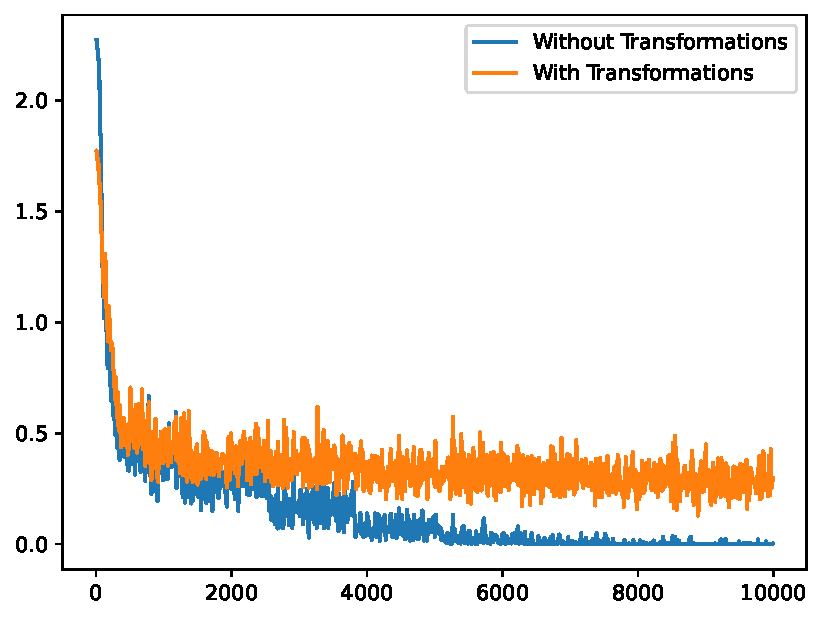
\includegraphics[width=\linewidth]{graphs/training/trans_img_training_loss_curve.pdf}
        \caption{Training Loss}
    \end{subfigure}
    \begin{subfigure}{0.48\textwidth}
        \centering
        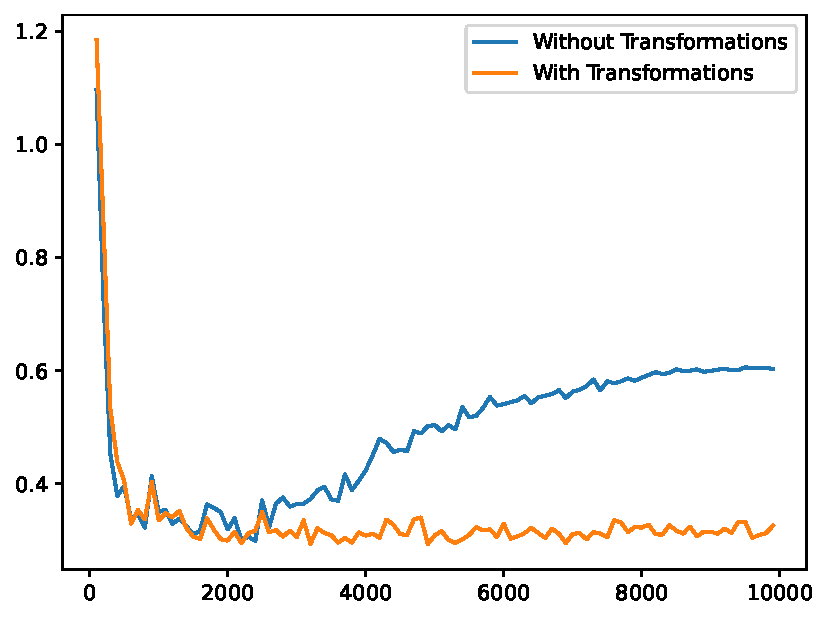
\includegraphics[width=\linewidth]{graphs/training/trans_img_eval_loss_curve.pdf}
        \caption{Evaluation Loss}
    \end{subfigure}
    \caption{Comparasion of \VIT Large training process with/without training transformations (first 10k steps only). A significant model overfit can be found without training transformations.}
    \label{fig:overfit}
\end{figure}

Doing transformations in Section~\ref{sec:pre_image} has effectively prevented overfitting. Figure~\ref{fig:overfit} clearly shows that without transformations, the model had a significant overfit after certain steps. The idea is that transformations make the task harder, so that models can learn more from the training data.

\subsubsection{Model Fine-tuning Details}\label{sec:finetuning_details}

\paragraph{Training Pipeline} We built the training pipeline using PyTorch. An abstract class \textsc{Model} was used as the interface, with other models inheriting from this class. By standardizing data loading and processing, we significantly reduced the time required to integrate individual models. Hugging Face Trainer \cite{wolf-etal-2020-transformers} and Weights \& Biases \cite{wandb_docs_2024} are integrated for training.

However, the pretraining vector for \CROP is stored in TensorFlow format. As a result, although it is still integrated into the pipeline, we used Keras to load and train the model.

\paragraph{Optimizer} We found no evidence that changing the optimizer affected the experimental results. Therefore, we decided to use AdamW \cite{loshchilov2019decoupledweightdecayregularization} for all models. Detailed optimizer config is listed in Appendix~\ref{appendix:optimizer_config}.

\paragraph{Learning Rate} The learning rate indeed affects the model's performance. We experimented with various learning rate schedules. We finally decided to use \texttt{ReduceLROnPlateau} for \VIT and \CROP, \texttt{CosineAnnealingWarmRestarts} \cite{loshchilov2016sgdr} for \CONV. Although we did not observe any effect from adjusting the warmup \cite{goyal2017accurate} steps, we still applied warmup with $100$ steps to the \CONV and \VIT in our final training. We didn't do warmup on \CROP. Detailed parameters is listed in Appendix~\ref{app:lr}.

\paragraph{Early Stopping} For \CONV and \VIT, since we can easily monitor and log in real-time through Weights \& Biases, we decided not to use Early Stopping. However, due to the difficulty of integrating Weights \& Biases with Keras, we can only output logs to the console when training \CROP, which makes real-time monitoring inconvenient. Therefore, we are considering using Early Stopping for \CROP.

\paragraph{Low-Rank Adaptation (LoRA)} When initially selecting models, we needed to conduct numerous experiments. To enable the simultaneous training of a large number of models with limited GPU resources, we integrated Low-Rank Adaptation (LoRA) \cite{hu2021lora}. This allowed us to quickly filter out underperforming models during the early stages of model selection, saving significant computational resources. However, during the final training phase, we removed this step, considering that LoRA might compromise the model's performance.

\paragraph{DDP and Batch Processing} Distributed Data Parallel (DDP) \cite{li2020pytorchdistributedexperiencesaccelerating} is used for our finalize training. To save time for training, we used $32\times 4\text{ (GPUs)}$ as our batch size.

\paragraph{Model Publishing and Submitting} Since the competition requires the submission of inference code rather than results, we have uploaded all the trained models to Hugging Face, which can be accessed by \href{https://huggingface.co/collections/pufanyi/sc4000-6717aaebf10b0e67e9a34a0d}{this link}. As the inference code needs to be offline, we have stored all the parameters in Kaggle Models for inference.


    \section{Merging Strategy and Error Analysis}\label{sec:voting}

\paragraph{Output Analysis}
% Individual Model Performance Analysis
We first analyze the individual model performance of \VIT{}, \CROP{}, and \CONV{} on the validation set.
\begin{figure}[htbp]
    \centering
    \begin{subfigure}{0.32\textwidth}
        \centering
        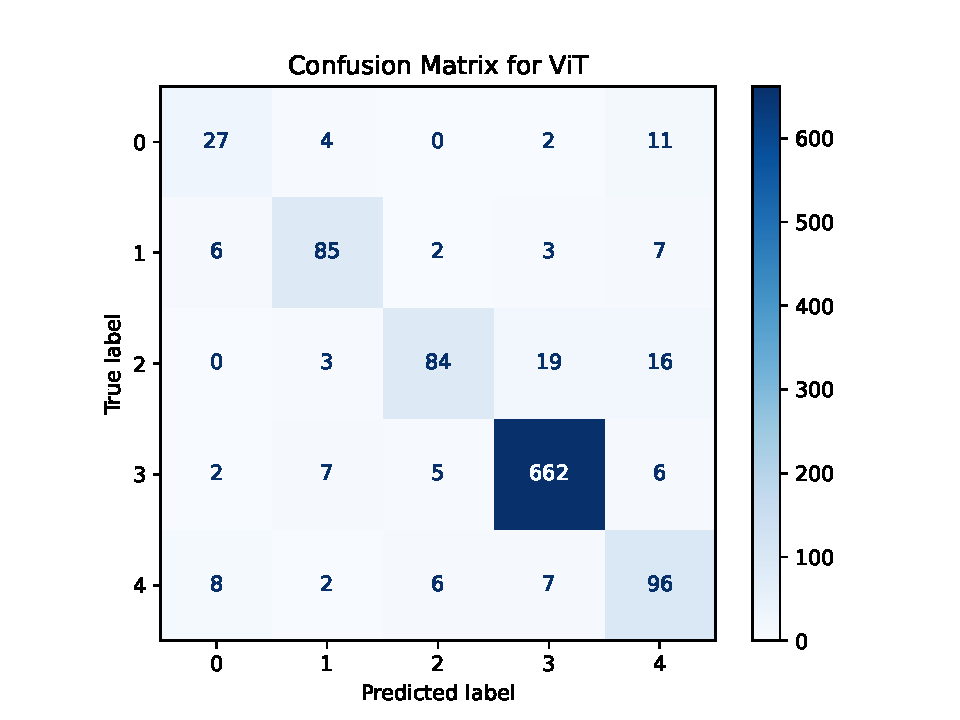
\includegraphics[width=\linewidth]{graphs/ModelMergeStudy/ViT.pdf}
        \caption{\VIT}
    \end{subfigure}
    \begin{subfigure}{0.32\textwidth}
        \centering
        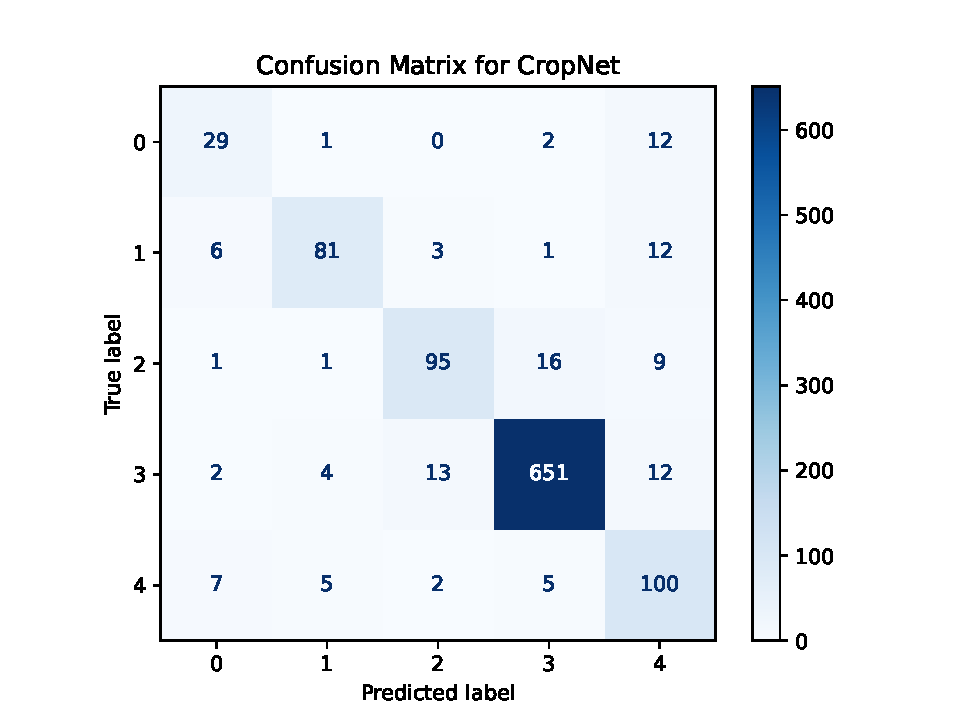
\includegraphics[width=\linewidth]{graphs/ModelMergeStudy/CropNet.pdf}
        \caption{\CROP}
    \end{subfigure}
    \begin{subfigure}{0.32\textwidth}
        \centering
        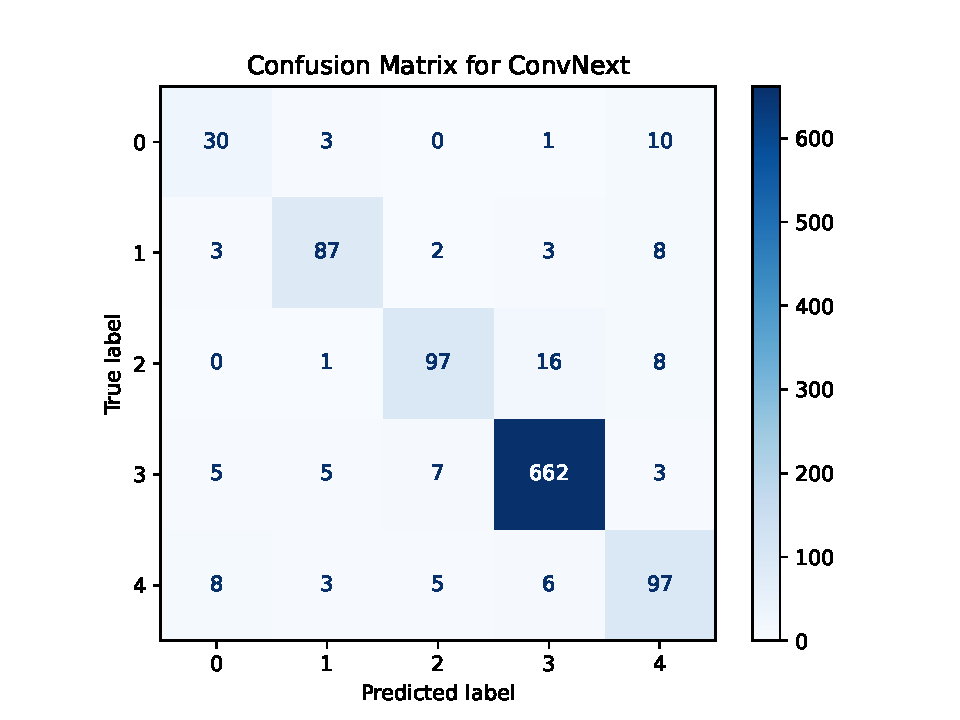
\includegraphics[width=\linewidth]{graphs/ModelMergeStudy/ConvNext.pdf}
        \caption{\CONV}
    \end{subfigure}
    \caption{Confusion Matrix for Three Models}
    \label{confusionMatrix}
\end{figure}

Fig~\ref{confusionMatrix} presents the confusion matrices for the three models: \VIT{}, \CROP{}, and \CONV{}. Each matrix illustrates how well the respective model classifies the validation dataset. The horizontal axis represents the label predicted by the model, while the vertical axis indicates the actual results. Thus, the diagonal elements indicate the correctly classified images, while the off-diagonal elements represent the misclassified instances.

The evaluation of the three models indicates that the dataset is imbalanced, with class 3 dominating the data. In addition, all models achieved their highest accuracy in class 3. Conversely, class 0 presents the greatest challenge, resulting in the lowest accuracy across all models. Among them, \CONV{} stands out for its overall accuracy, excelling in classes 0, 1, 2, and 3, though \CROP{} slightly performs better in class 4. Notably, \CROP{} and \VIT{} demonstrate complementary strengths, with \CROP{} performing better in classes 0, 2, and 4, while \VIT{} shows an advantage in classes 1 and 3. Therefore, combining these models together could yield better results.
\paragraph{Hard Voting}
Hard voting, also known as majority voting, involves each model casting a "vote" for a specific class, with the final outcome determined by the majority of votes from all models. This method does not take into account the probabilities associated with each model's prediction. As demonstrated in Algorithm \ref{alg:hardvote}, we implemented hard voting based on the three models discussed previously. In the event of a tie, we have observed that we will default to the result from \CONV{} as the final outcome.


% persudo code
\begin{algorithm}[ht]
\SetAlgoLined
\KwData{Input data $X$, Models \CONV{}, \CROP{}, \VIT{}}
\KwResult{Final prediction $y$}
\caption{Hard Voting Ensemble with Tie-Breaker}
\label{alg:hardvote}
$y_{\text{conv}} \gets$ \CONV.predict($X$)\;
$y_{\text{crop}} \gets$ \CROP.predict($X$)\;
$y_{\text{vit}} \gets$ \VIT.predict($X$)\;
$votes \gets \{y_{\text{conv}}, y_{\text{crop}}, y_{\text{vit}}\}$\;
$count \gets$ count occurrences of each class in $votes$\;
\eIf{maximum count in $count$ is unique}{
    $y \gets$ class with maximum count in $count$\;
}{
    $y \gets y_{\text{conv}}$ \tcp*{Tie-breaker: choose \CONV{} prediction}
}
\Return{$y$}
\end{algorithm}

As shown in Fig~\ref{fig: hard voting}, the hard voting algorithm allowed us to combine the strengths of each individual model, reducing wrong predictions and enhancing overall accuracy. However, hard voting could also lead to suboptimal results when models vary significantly in accuracy. For example, if a model is indecisive between two classes, using its hard vote may lead to an inaccurate result.

\paragraph{Soft Voting}

In contrast, soft voting addresses this issue by calculating the probability scores from each model's predictions. As illustrated in Fig~\ref{fig:cdf}, we compared the probability differences in cumulative distribution between the ground truth and predicted variables. The results indicate that approximately $20\%$ shows no significant difference, while $40\%$ shows only minor differences. This suggests that soft voting could also yield favorable results.

We implemented a soft voting algorithm as shown in Algorithm~\ref{soft voting}. Each model predicts a corresponding probability for each class. Then, we sum these probabilities to calculate an overall probability. Finally, we select the class with the highest overall probability as the final predicted result.

\begin{figure}
    \centering
    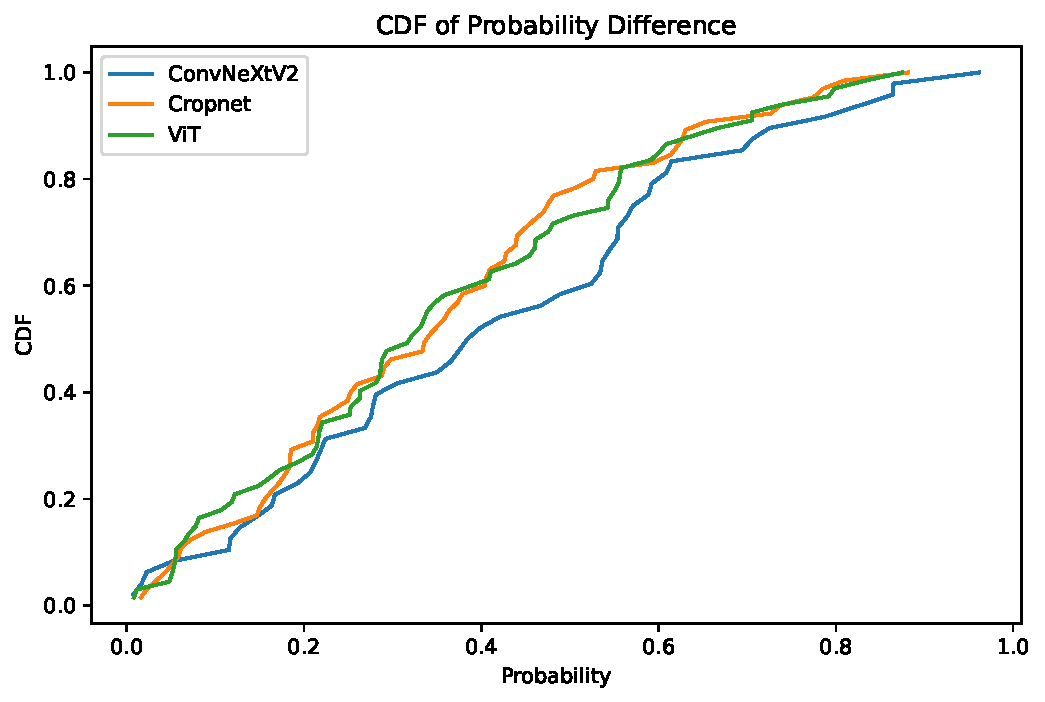
\includegraphics[width=0.7\linewidth]{graphs/ModelMergeStudy/cdf}
    \caption{CDF for Probability Difference}
    \label{fig:cdf}
\end{figure}

\begin{algorithm}[ht]
\SetAlgoLined
\KwData{Input data $X$, Models \CONV{}, \CROP{}, \VIT{} with probability outputs}
\KwResult{Final prediction $y$}
\caption{Soft Voting Ensemble}
\label{soft voting}
$P_{\text{conv}} \gets$ ConvNet.predict\_proba($X$) \tcp*{Probability output of ConvNet}
$P_{\text{crop}} \gets$ CropNet.predict\_proba($X$) \tcp*{Probability output of CropNet}
$P_{\text{vit}} \gets$ ViT.predict\_proba($X$) \tcp*{Probability output of ViT}
$P_{\text{total}} \gets P_{\text{conv}} + P_{\text{crop}} + P_{\text{vit}}$
$y \gets \arg\max(P_{\text{total}})$ \tcp*{Select class with highest summed probability}

\Return{$y$}

\end{algorithm}

\paragraph{Conclusion}

\begin{figure}[t]
    \centering
    \begin{subfigure}{0.45\textwidth}
        \centering
        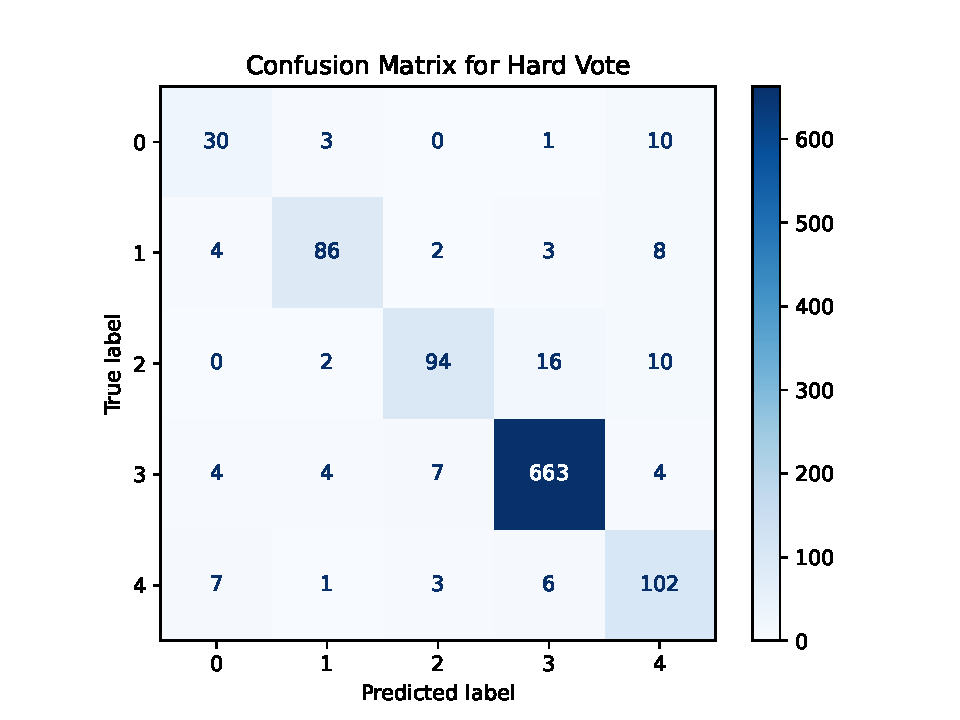
\includegraphics[width=\linewidth]{graphs/ModelMergeStudy/Hard Vote.pdf}
        \caption{Hard Voting}
        \label{fig: hard voting}
    \end{subfigure}
    \begin{subfigure}{0.45\textwidth}
        \centering
        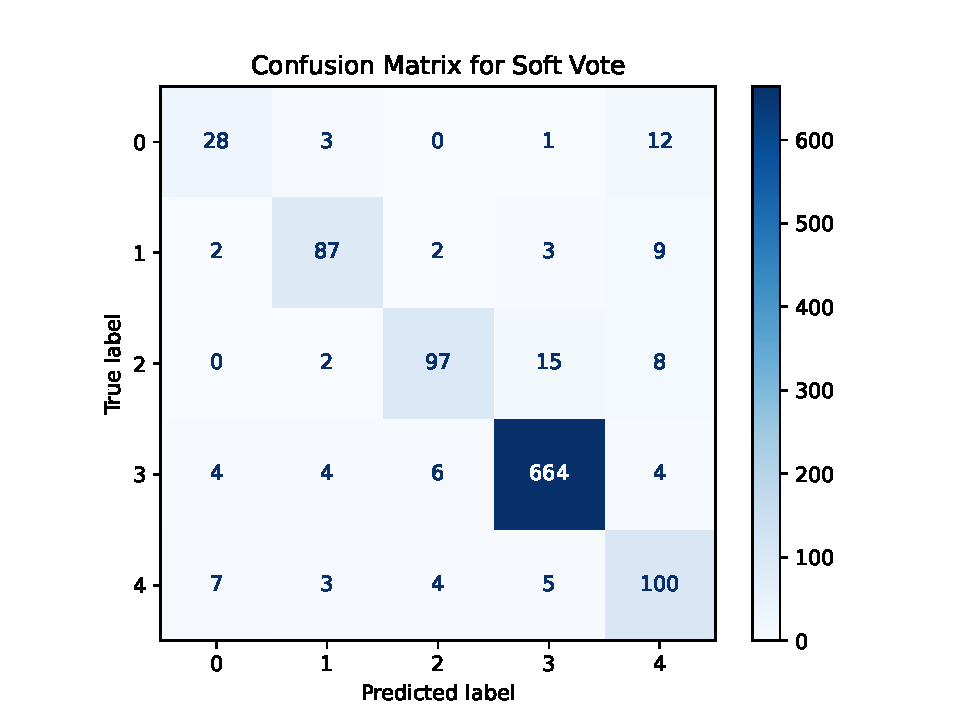
\includegraphics[width=\linewidth]{graphs/ModelMergeStudy/Soft Vote.pdf}
        \caption{Soft Voting}
        \label{fig: soft voting}
    \end{subfigure}
    \caption{Confusion Matrix for Hard Voting and Soft Voting}
    \label{hard soft confusionMatrix}
\end{figure}

Fig~\ref{hard soft confusionMatrix} shows the confusion matrix for both hard and soft voting. Both algorithms share the common advantage of effectively improving overall accuracy. However, there are slight differences in performance across specific classes. Compared to soft voting, hard voting yields more accurate predictions for classes 0 and 4 but performs less effectively for classes 1, 2, and 3. Overall, soft voting achieves a higher accuracy rate.

Compared to hard voting, soft voting benefits from the use of more granular probability scores, which reduces sensitivity to wrong predictions, better handles class imbalances in the original data, and offers improved generalization ability. Therefore, we have decided to use soft voting as our chosen method.

Our soft voting method reached $90.79\%$ (rank 17/3901) in the public benchmark.

\section{Further Improvement in The Merging Process}

Besides Hard Voting and Soft Voting discussed in Section \ref{sec:voting}, we proposed a voting method called \textit{Soft Voting with Confidence}. The general idea is that if a model generates more extreme probabilities, it should be more confident, and we should assign it greater voting weight. Conversely, if the model's results are ambiguous, we should reduce its weight.

We define a \textbf{confidence} $c(p)$ as a function
\begin{equation}
    c: [0, 1] \to [0,\infty)
\end{equation}
with the following properties:
\begin{enumerate}
    \item $c(0) = c(1) = 1$;\label{prop:eq1}
    \item $c$ is continuous in $[0, 1]$;\label{prop:cont}
    \item $c$ is a quasiconvex function, which means:\begin{equation}
        \forall x_1, x_2, t\in [0, 1]^3, c(tx_1 + (1-t)x_2)\le \max\{c(x_1), c(x_2)\}
    \end{equation}\label{prop:convex}
\end{enumerate}
Property~\ref{prop:eq1} suggests that if the model predicts probability $0$ or $1$, it should have full confidence. Property~\ref{prop:cont} ensures a slight change in prediction won't affect too much. Property~\ref{prop:convex} defines the shape of the confidence function.

We define the voting weight
\begin{equation}
w(p) = p\cdot c(p)
\end{equation}

So the final value is
\begin{equation}
    v_{\text{total}}(i) = \sum_{m\in\text{models}}w(p_m(i))\cdot p_m(i) = \sum_{m\in\text{models}}\left(p_m(i)\right)^2\cdot c(p_m(i))
\end{equation}

We selected confidence functions
\begin{equation}
    c(p) = \frac{\cosh(2p-1)}{\cosh(0)} = \frac{e^{2p-1}+e^{-2p+1}}{e +e^{-1}}
\end{equation}
in our model.


    % \section{Results}




    \section{Conclusion}

This project focuses on developing models for classifying cassava leaf diseases using advanced machine-learning techniques. It addresses challenges such as data imbalance and noise found in real-world datasets. By employing data augmentation, we combine traditional data pre-processing methods with advanced techniques like the Segment Anything Model. Additionally, we evaluated and integrated results from various model architectures, including \VIT, \CONV, and \CROP. By utilizing a soft voting algorithm, we were able to enhance classification accuracy and generalization.

Finally, our model achieved $90.95\%$ (Rank $4 / 3901$, Top $0.10\%$) on Public Benchmark and $90.60\%$ (Rank $2 / 3901$, Top $0.05\%$) on Private Benchmark. Detailed submission results and codes can be accessed in Appendix~\ref{app:submission_details}.

	
	\bibliographystyle{plain} % or another style like apalike, abbrvnat, etc.
	\bibliography{references/ref} % assumes you have a references.bib file
	
	
	
	%%%%%%%%%%%%%%%%%%%%%%%%%%%%%%%%%%%%%%%%%%%%%%%%%%%%%%%%%%%%
	
	\newpage
	\appendix

    \section{Training Details}

\subsection{Learning Rate}\label{app:lr}

Table~\ref{tab:learning_rate} lists learning rate configs for each model. For \VIT and \CONV, we have $\text{warmup}=500$. For \CROP, we don't have warmup steps.

\begin{table}[ht]
    \centering
    \begin{tabular}{c|cccc}
    \toprule
       \textbf{Model} & \textbf{Learning Rate}\tablefootnote{Intial learning rate, do not include warmup. So the actual Intial learning rate is $\frac{\text{Learning Rate}}{\text{Warmup Steps}}$.} & \textbf{Scheduler} & \textbf{Details} \\
    \midrule
        \VIT & $10^{-4}$ & ReduceLROnPlateau & $\begin{cases}\text{patience}=10\\\text{factor}=0.5\\\text{min\_lr}=5\times 10^{-6}\end{cases}$  \\
    \midrule
        \CONV & $10^{-4}$ & CosineAnnealingWarmRestarts & $\text{num\_cycles} = 0.5$\\
    \midrule
        \CROP & $10^{-5}$ & ReduceLROnPlateau & $\begin{cases}\text{patience}=5\\\text{factor}=0.5\\\text{min\_lr}=10^{-8}\end{cases}$  \\
    \bottomrule
    \end{tabular}
    \caption{Learning Rates Details for Each Models}
    \label{tab:learning_rate}
\end{table}

\subsection{LoRA Cofig}

In model selection period, we performed low-rank adaptation (LoRA) \cite{hu2021lora} for all experiments. We used the same LoRA config for all models to achieve the fairness.

We applied LoRA on all linear layers. Low rank matrices $A$ and $B$ are generated with the same method as in \cite{buyukakyuz2024olora}. The rank matrices are set to $8$, and the $\alpha$ parameter for LoRA scaling is set to $8$.

\subsection{Optimizer Config}\label{appendix:optimizer_config}

As section \ref{sec:finetuning_details} mentioned, we found no evidence that changing the optimizer affected the experimental results. So we use AdamW with hyperparameter $\beta_1=0.9, \beta_2=0.999, \epsilon=10^{-8}$ for all training processes.

\section{Submission Details}\label{app:submission_details}

We submitted our results to \href{https://www.kaggle.com/competitions/cassava-leaf-disease-classification/submissions}{Kaggle}.

Our final submission code can be found \href{https://github.com/pufanyi/SC4000/blob/main/submission/final_submission.ipynb}{here}.

Our final submission achieved $90.95\%$ (Rank $4 / 3901$, Top $0.10\%$) on Public Benchmark and $90.60\%$ (Rank $2 / 3901$, Top $0.05\%$) on Private Benchmark, shown in Figure \ref{fig:submission}, \ref{fig:public_lb} and \ref{fig:private_lb}.

\begin{figure}[H]
    \centering
    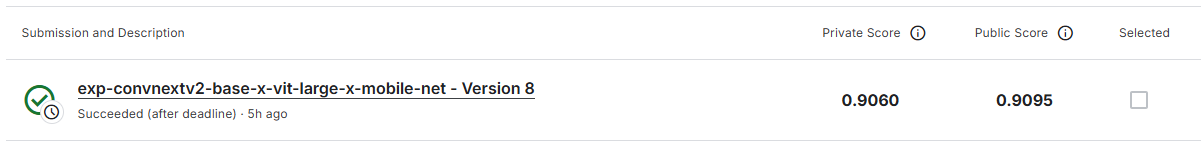
\includegraphics[width=1\linewidth]{graphs/appendix/results.png}
    \caption{Submission Results}
    \label{fig:submission}
\end{figure}

\begin{figure}[H]
    \centering
    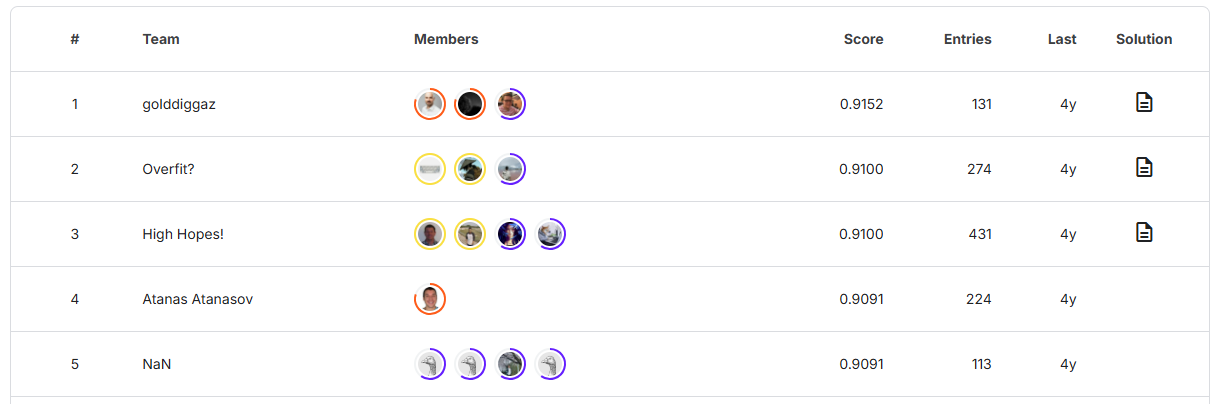
\includegraphics[width=1\linewidth]{graphs/appendix/publiclb.png}
    \caption{Public Leaderboard}
    \label{fig:public_lb}
\end{figure}

\begin{figure}[H]
    \centering
    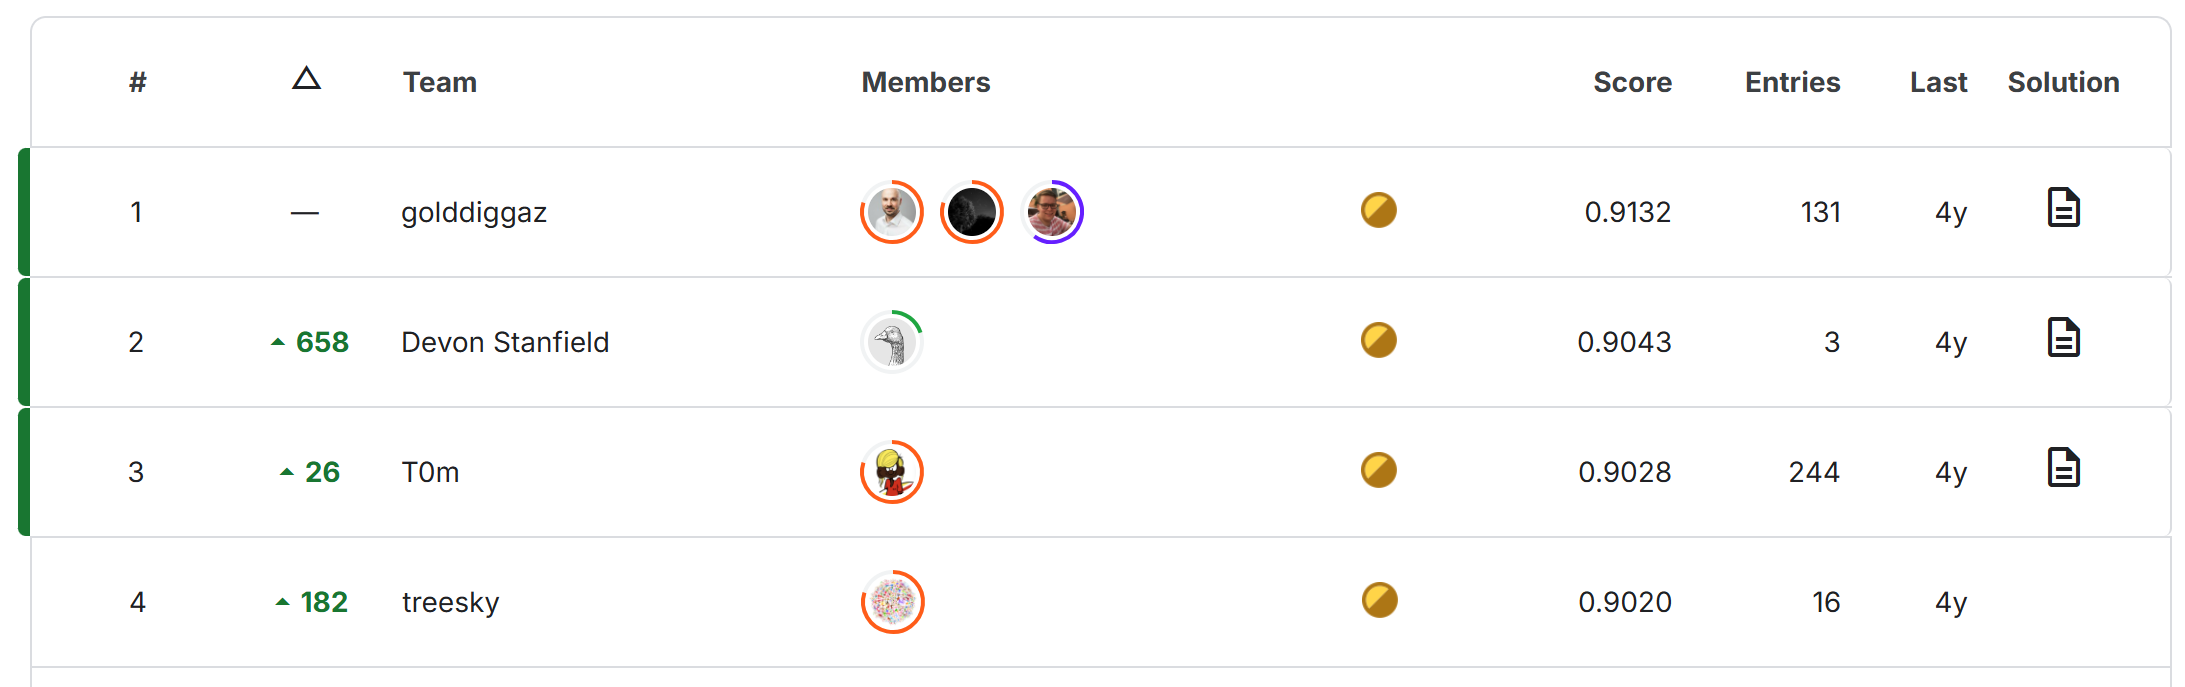
\includegraphics[width=1\linewidth]{graphs/appendix/privatelb.png}
    \caption{Private Leaderboard}
    \label{fig:private_lb}
\end{figure}
	
	
\end{document}